%%%%%%%%%%%%%%%%%%%%%%%%%%%%%%%%%%%%%%%%%%%%%%%%%%%%%%%%%%%%%%%%%%%%%%%%%%%%%%%%
%2345678901234567890123456789012345678901234567890123456789012345678901234567890
%        1         2         3         4         5         6         7         8

\documentclass[letterpaper, 10 pt, conference]{ieeeconf}  % Comment this line out if you need a4paper

%\documentclass[a4paper, 10pt, conference]{ieeeconf}      % Use this line for a4 paper

\IEEEoverridecommandlockouts                              % This command is only needed if 
                                                          % you want to use the \thanks command

\overrideIEEEmargins                                      % Needed to meet printer requirements.

%In case you encounter the following error:
%Error 1010 The PDF file may be corrupt (unable to open PDF file) OR
%Error 1000 An error occurred while parsing a contents stream. Unable to analyze the PDF file.
%This is a known problem with pdfLaTeX conversion filter. The file cannot be opened with acrobat reader
%Please use one of the alternatives below to circumvent this error by uncommenting one or the other
%\pdfobjcompresslevel=0
%\pdfminorversion=4

% See the \addtolength command later in the file to balance the column lengths
% on the last page of the document

\usepackage{epsfig}
\usepackage{float}
\usepackage{threeparttable}
\usepackage{subfigure}
\usepackage{url}

% The following packages can be found on http:\\www.ctan.org
%\usepackage{graphics} % for pdf, bitmapped graphics files
%\usepackage{epsfig} % for postscript graphics files
%\usepackage{mathptmx} % assumes new font selection scheme installed
%\usepackage{times} % assumes new font selection scheme installed
\usepackage{amsmath} % assumes amsmath package installed
\usepackage{amssymb}  % assumes amsmath package installed

\usepackage{bigstrut,multirow}
	
\usepackage[colorlinks=false, pdfborder={0 0 0}]{hyperref}
\usepackage{cleveref}
\crefname{figure}{fig}{figs}

\usepackage{microtype}


\title{\LARGE \bf
Data-efficient CNN-based Multi-robot Map Building with Panoramic Camera.
}


% \author{ Jincheng Yu$^{1}$,  Zhilin Xu$^{1}$, Feng Gao$^{1}$, Zhaoliang Zhang$^{1}$ and Yu Wang$^{1}$ % <-this % stops a space
% \thanks{*This work was not supported by any organization} % <-this % stops a space
% \thanks{$^{1}$Electronic Engineering Department,
%         Tsinghua University, Beijing, China
%         {\tt\small yjc16@mails.tsinghua.edu.cn, yu-wang@tsinghua.edu.cn}}%
% }


\begin{document}

\maketitle
\thispagestyle{empty}
\pagestyle{empty}


%%%%%%%%%%%%%%%%%%%%%%%%%%%%%%%%%%%%%%%%%%%%%%%%%%%%%%%%%%%%%%%%%%%%%%%%%%%%%%%%
\begin{abstract}
Multi-robot map building of unknown environments is a fundamental problem for multi-robot autonomous robotics. 
Different from single-robot's huge on-board communication bandwidth, the limited communication resources between robots becomes the bottleneck of the multi-robot map building.
In order to do multi-robot map building in communication constrained environments, this paper proposes a data-efficient map representation and merging method based on topology map, called PRET.
% (Place Representor Embedded Topology map)
PRET uses CNN to generate place representor of each new comming place and embeds the representor to the topology map.
Based on the representors, the topology maps of different robots can be easily shared and merged with little communication resources.
Compared with the tranditional grid map. The data transfer is reduced by ?\%. The navigation path is only ?\% higher than the grid map. %结果稍微丰富下
\end{abstract}

\section{Introduction}
\label{sec:intro}

With the development of algorithms and computation platforms, a single moving robot can navigate and build map in a novel environment. 
Limited by the perception range, the system capability of a single robot is not sufficient to deal with tasks in complex environments.
The cooperation of different robots can greatly improve the system capability, and the multi-robot system is a promising research field.

Distributed Simultaneously Localization and Mapping (DSLAM)~\cite{corah2019communication, cieslewski2018data}, which provides the status of different robots and the environment, is a fundamental problem for multi-robot systems, including multi-robot navigation \cite{tanner2005towards} and rescue \cite{baxter2007multi}. As illustrated in \Cref{fig:DSLAMframe}, there are three function thread on each robot, Visual Odometry (VO), Map Building (Map) and Place Recognition (PR). VO reads two time adjacent input images and calculates the relative pose between these images, and finial produces the trajectory of the robots. PR generates compact image representation to produce the candidate place recognition matches between different robots. Map thread records trajectory and builds the environment into local map.

\begin{figure*}[t]
    \begin{minipage}[t]{0.3\linewidth}  
    \centering
    \subfigure[ DSLAM framework. Each frame is fed to VO to calculate trajectory. The local map is build based on the trajectory. Some key frames are fed to PR to encode the scenes into descriptors for inter-robot scene matching. When the same scene is detected with different robots, the local maps of these robots are merged into global map. In this work, we adopt panoramic camera and CNN to DSLAM system. Use topology map for both PR and Map.
    ] {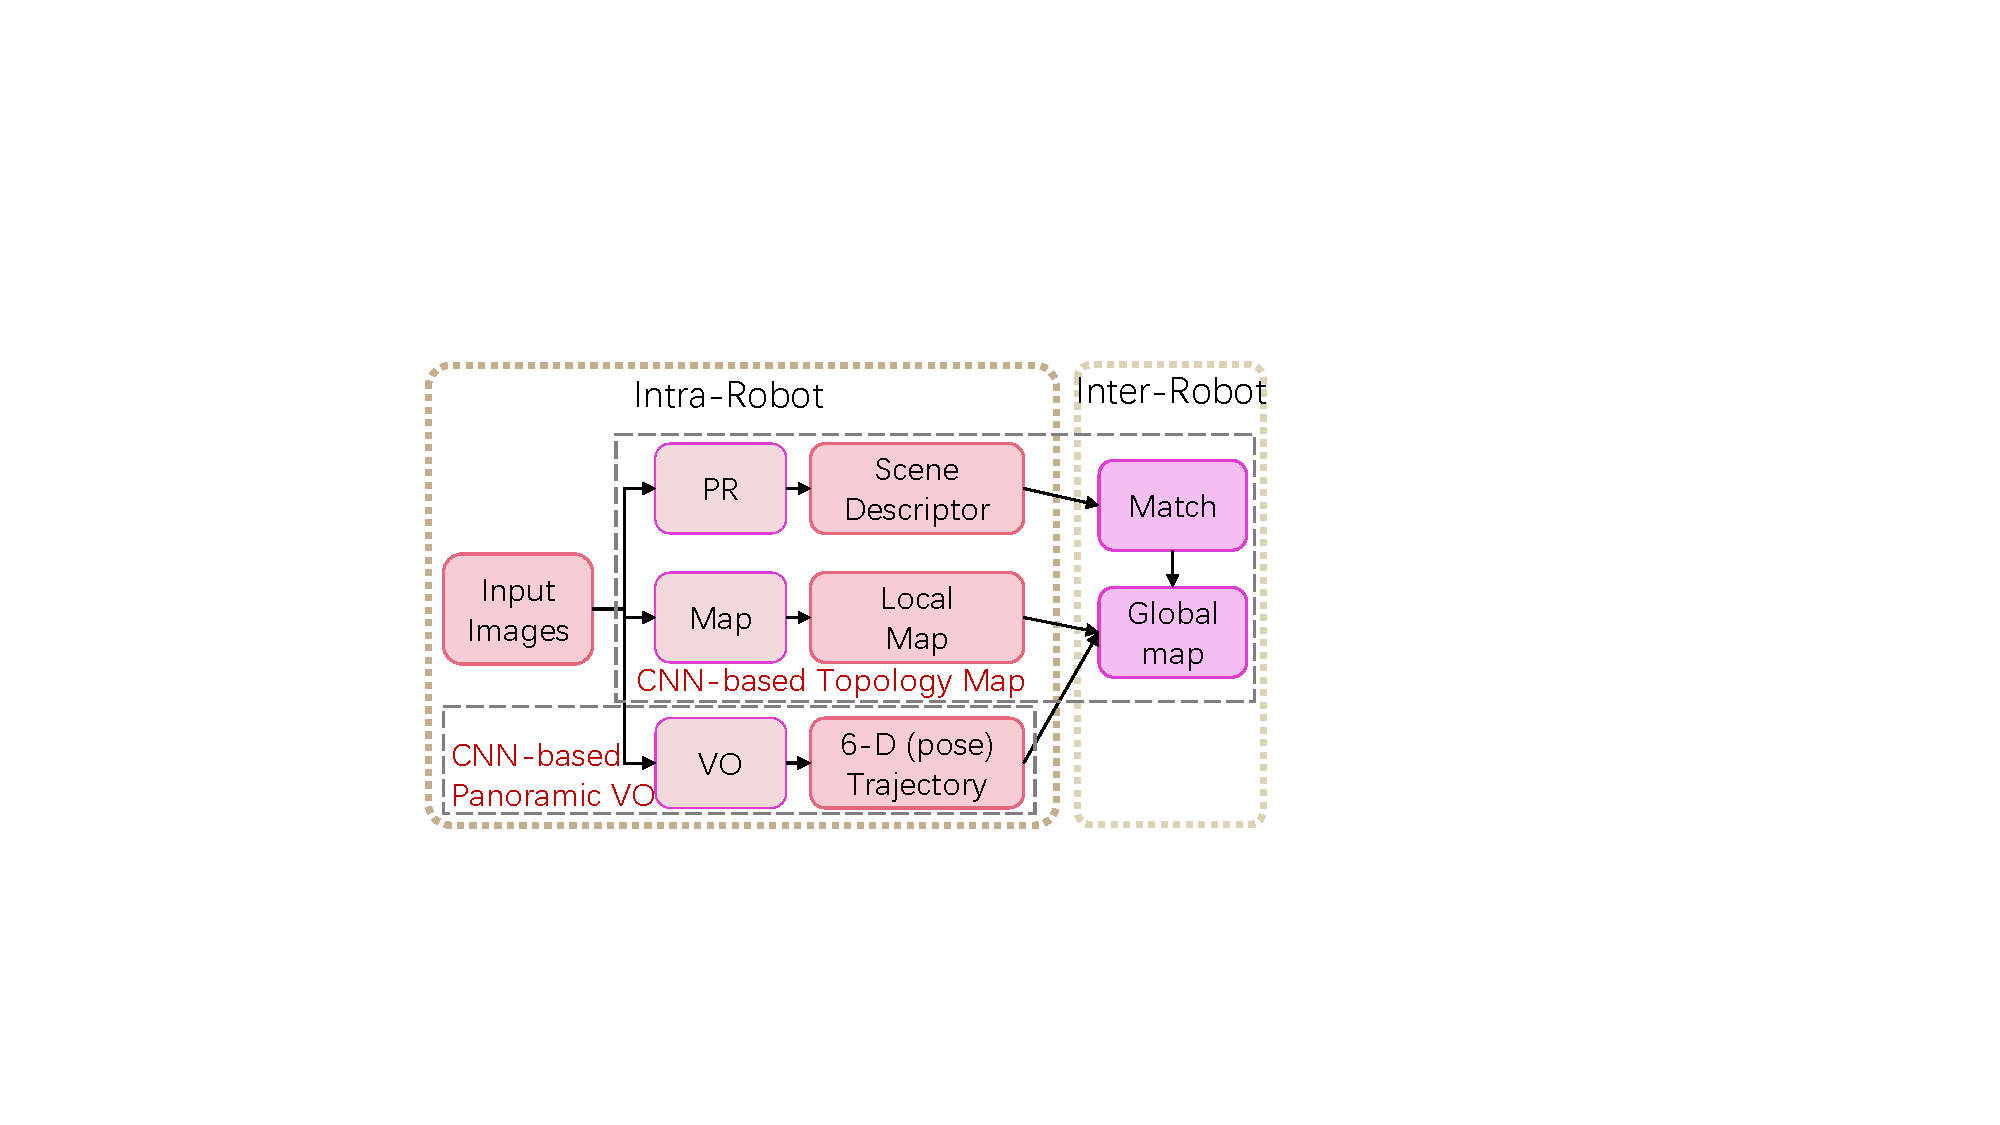
\includegraphics[width=0.95\textwidth]{fig/DSLAMframe.pdf}\label{fig:DSLAMframe}}
    \end{minipage}
    \begin{minipage}[t]{0.7\linewidth}  
    \centering  
    \subfigure[ Our CNN-based DSLAM system with panoramic camera. For VO, we use CNN to calculated the poses between different splited panoramic image frames \textcircled{1} and use graph optimization to fine-tune the camera pose of adjacent time. For Map and PR, we adopt CNN to generate descriptors \textcircled{3} for place recognition and build topology map based on the descriptors \textcircled{4}. We derectly match the topology map between robots \textcircled{5} and merge the local topology map \textcircled{6}.
    ] {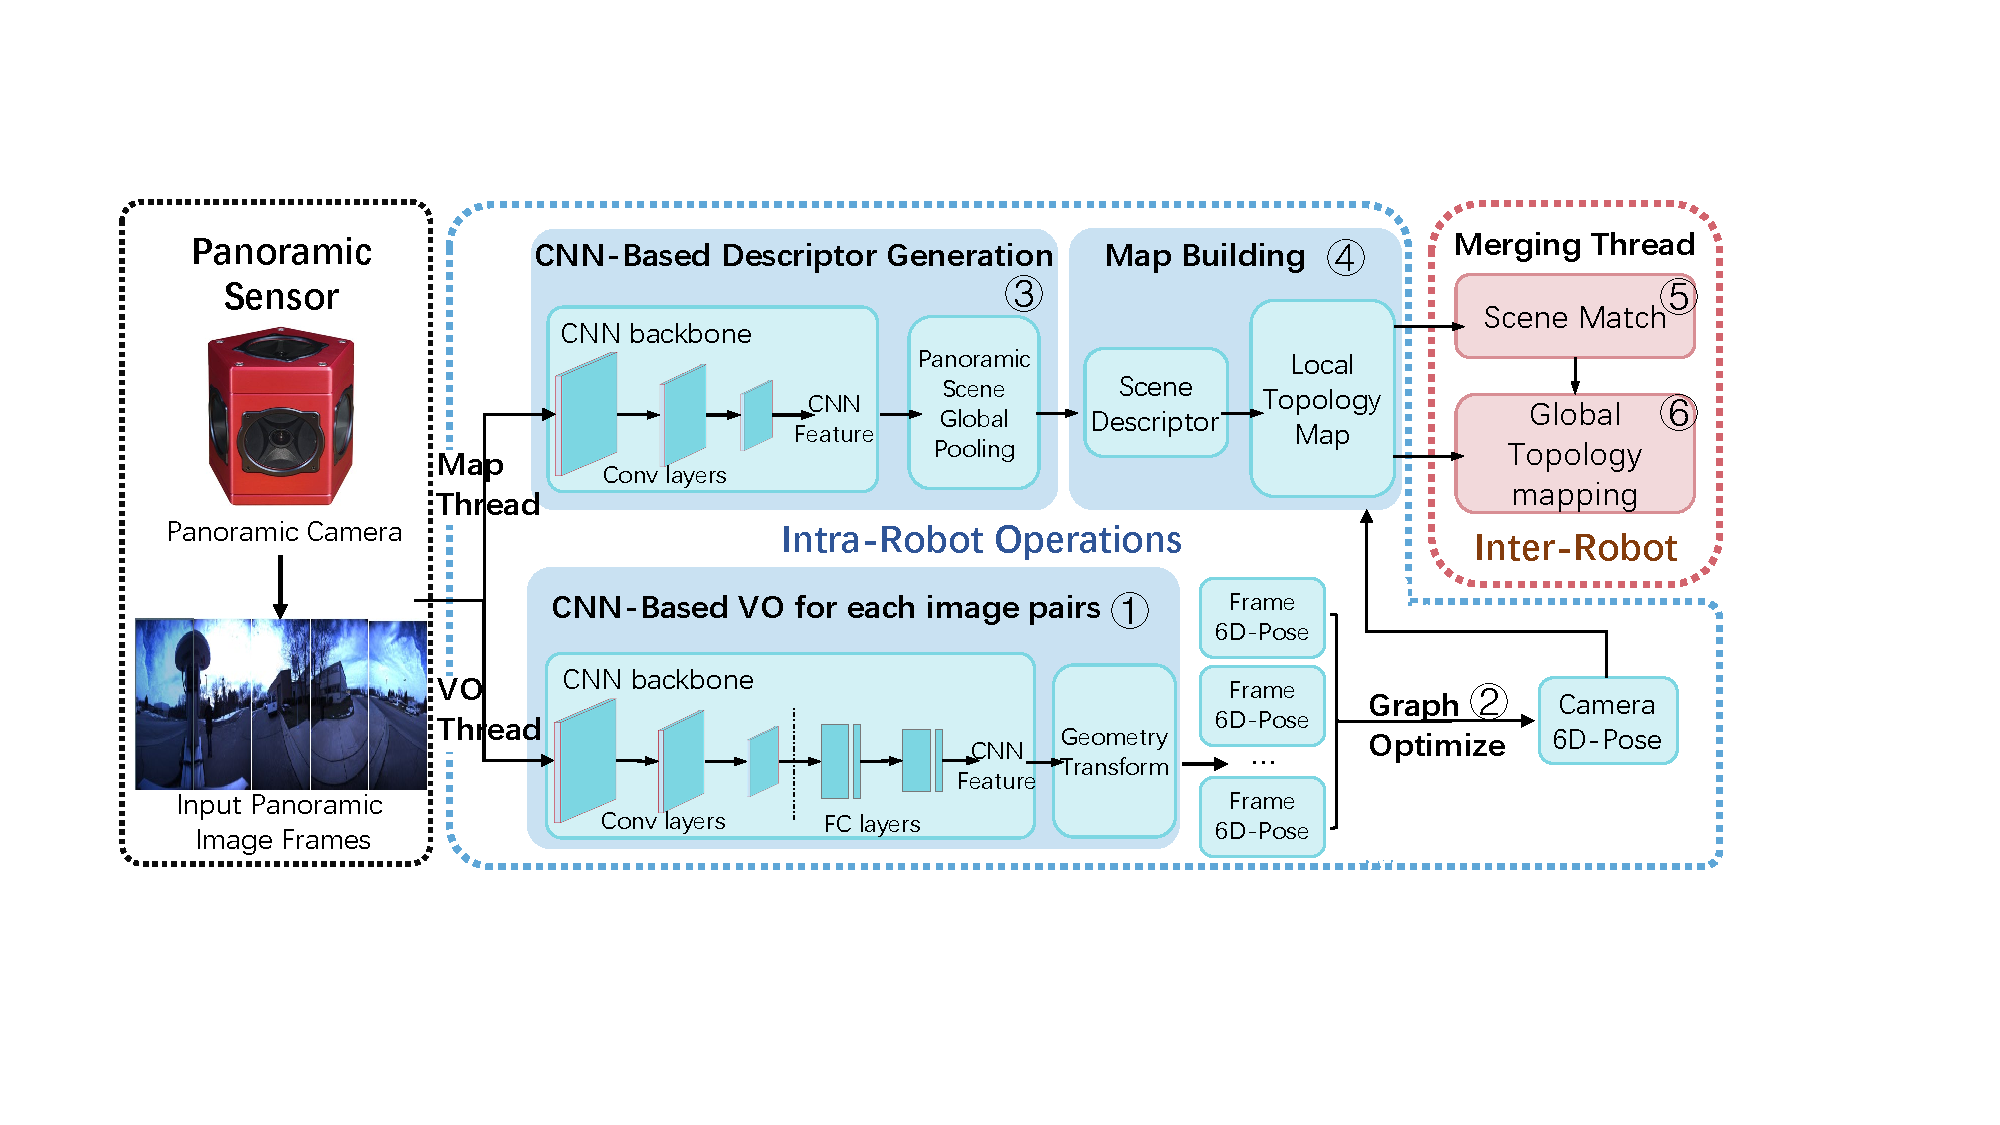
\includegraphics[width=0.95\linewidth]{fig/framework.pdf}\label{fig:framework}} 
    \end{minipage}
    \caption{DSLAM overview. \Cref{fig:DSLAMframe} shows the general DSLAM framework. \Cref{fig:framework} shows our CNN-based method with panoramic camera and topology map.
    }
\label{fig:overview}
\end{figure*}



\bibliographystyle{IEEEtran}
\bibliography{src/fpgaslam}

\end{document}
